% filepath: /home/jinm/eda/solver/project/report.tex

\documentclass[12pt]{ctexart}

% 包含常用包
\usepackage[utf8]{inputenc}    % 输入编码
\usepackage{amsmath, amssymb} % 数学符号
\usepackage{graphicx}          % 插入图片
\usepackage{hyperref}          % 超链接
\usepackage{geometry}          % 页面布局
\usepackage{fancyhdr}          % 页眉页脚
\usepackage{cite}              % 引用
\usepackage{listings}          % 代码高亮
\usepackage{xcolor}            % 颜色

% 页面设置
\geometry{a4paper, margin=1in}

% 页眉页脚设置
\pagestyle{fancy}
\fancyhf{}
\fancyhead[L]{项目报告}
\fancyhead[R]{\thepage}

% 代码样式
\lstset{
    language=C++,
    basicstyle=\ttfamily\small,
    keywordstyle=\color{blue},
    stringstyle=\color{orange},
    commentstyle=\color{gray},
    breaklines=true,
    numbers=left,
    numberstyle=\tiny\color{gray},
    stepnumber=1,
    numbersep=5pt,
    frame=single,
    captionpos=b
}

\title{eda报告}
\author{马晋}
\date{\today}

\begin{document}

\maketitle

\begin{abstract}
    这是大作业报告,我实现了一个eda算法,成功的对输入的def文件进行了时钟树综合。并且给出综合结果。
    我没有在比赛之前完成,但是如果没有出现剑走偏锋专门优化buffer\_count或total\_latency或skew的情况,我认为我的算法大概率是可以进决赛的。
    就我与此问题本班其他队对比的结果,我的算法的performance最好:体现在:时间上,我的算法skew可以100\%保证在45以内,并且在10(cts\_problems)+3(pre\_submit)中只有1个超过40(44),其余全都在35以下。
    而且我的average\_delay基本是最大那个距离的delay(但是由于插入了两到三个buffer,所以会有50到75的偏差)。
    并且我的聚类算法较佳,以至于在iterative\_cluster的时候,能非常近似的到达只考虑max\_fanout(不考虑偏离中心的bound)的误差,根据我从另一队eda展示的结果,我推测最终评测的case应该是在这些case中评测规模较大的,并且第一个应该是类似于pre\_submit的case1,
    总结:越是规模大的case我越存在优势,但是即使规模小的case我的performance也很强(此时buffer\_count可能稍微大一点点(约100~200)),并且我的程序具有极大的稳定性。
\end{abstract}

\tableofcontents
\newpage

\section{引言}
通过这个project,我认识到,完善和修改不能一蹴而就,最好分多步,循序渐进的构造。
\section{创新点}
project的创新点如下\\
1.分块操作,这是一个非常重要的方式,我对比了没有分块与分块的算法,时间上加速了10到20倍 \\
2.参数可配置化,全都在parameter.cpp中,其中包含FF聚类的初始数量,大小,以及最后生成逻辑过程中对于时间skew的忍受度,等等。我将前面部分和后面部分解耦合,采用不同的配置,
目前,我已经在当前情况下,将配置调整到了一个比较优的条件,实际上,还可以进一步优化,即根据文件规模与密度进行优化。(而且在我的代码的基础上很容易实现)\\
3.关于聚类,实际上,我的聚类效果已经接近极限,我的聚类是实现在偏移中心距离不超过max\_bound下的聚类,经过我的验证,这个聚类的约束确实是非常完美的,可以给出数据,在parameter.cpp中,将bound和max\_bound改成2000000(那么此时完全是fanout约束),我发现需要3200个点的在只有fanout约束下要3000个点,这说明,我的聚类算法是非常优化的。\\
4.我的overlap算法是基于优先队列加查找的,实际上,这是我考察了题目得出的综合结果,这一定是近乎最优的方案,一方面,它搜索的范围很广,另一方面,它能找到偏离中心不会太远的点,,不会因为离群点而倒是成为时间优化的瓶颈。所以实际上,可视化后可以看见生成的图很漂亮,并且可以看见重合度非常低。根据最终cts\_checker的结果,我把所有的overlap优化到了0.2\%以下 \\
5.基于我对题目的观察,我对二次距离进行了最优的优化,这是题目中非常重要的性质    \\
6.实际上,我在算法中尽量保证了稳当性,使得尽量在一些极端情况下都能运行,比如,highlevelcluster中,我实际上是反复的迭代直到终止,而按照测试样例,实际上只用迭代一次。    \\
7.我完成了可视化,老师可以通过output.svg查看   \\
8.我分析了很多程序中的问题,用gdb -g debug    \\
9.我已经为老师和学长写好了自动化脚本,方便老师和学长测试最终结果 


\section{方法}
方法已经在ppt中介绍了,中心思想是利用可以确定的最远的延迟,在这个基础上,调整其他的buffer贴近这个最远的延迟。
然而事实上,问题远不止这么简单:
怎样聚类?
怎么减小overlap?
怎么保持约束?
怎么debug?
发现原来的程序不够好,我要做改动,我该怎么做?(尽量等效)
\section{cluster}
我的聚类用的是循环的迭代聚类,它会循环自动的迭代找到最小的聚类数量,一方面在这个过程中fan\_out不会超出范围。另一方面这个过程中bound不会超出范围.
此外,这个算法的聚类结果与无约束下的聚类结果非常相近,这是因为我在聚类的时候,我会根据fan\_out的大小,选择一个合适的bound,这个bound是根据我对题目的观察得出的。\\
\subsection{overlap}
对于overlap我用的优先队列,经过我的测试,我的几乎所有case的overlap都在\%0.2左右.
\subsection{floorplan}
我以最新解决的一个问题为例,可以从中窥出实际上有很多的细节问题:
\begin{figure}[h]
    \centering
    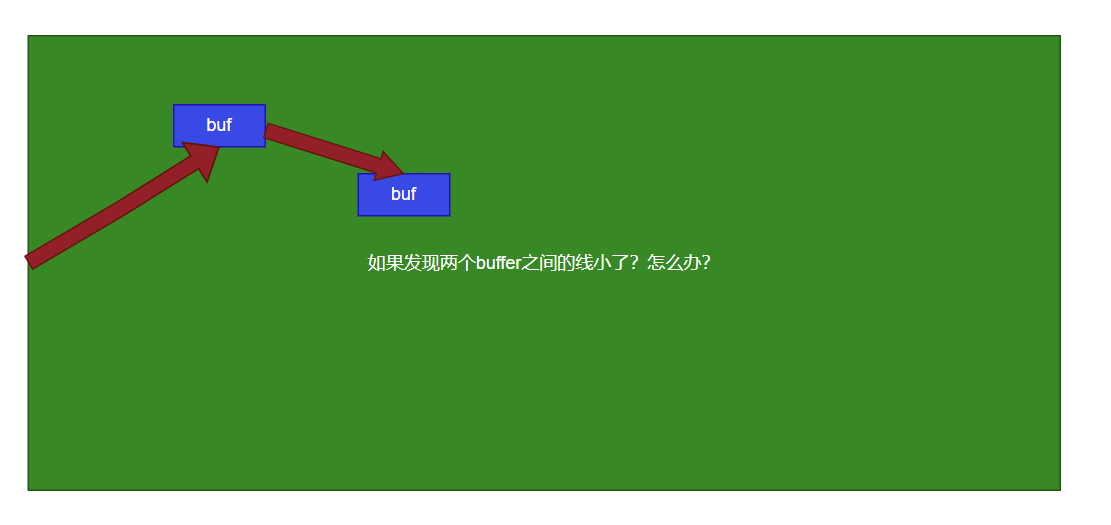
\includegraphics[width=0.8\textwidth]{buf-floorplan.png}
    \caption{BUF}
    \label{fig:example}
\end{figure}
如图所示,这是一个buffer的floorplan,现在我希望把后面的buffer延迟调整到与前面找到的最大值尽量相同从而减少skew:
如果我沿着两个buf的连线,找到一个buf作为中转(这样算很容易且不用分类讨论),相连,则极有可能最后出现这个buf的位置超出floorplan。
但是不这样的话,为了找到中转buf(使得最后的buf延迟接近于我希望的延迟),似乎要讨论很多的可能性(因为是曼哈顿距离,和绝对值相加,所以需要有很多的分类讨论),从而导致问题一下子复杂了很多。
但是,如果结合实际,如果buf位连线的latency小了,这个一定是发生在左边,从而隐式的推断出此时x很小的事实,那么我可以选择找x的位置,此时我预期是不会超过floorplan的,
至于y,因为我要计算两个buf与中转buf的曼哈顿距离,似乎又要分类计算了,但是发现如果选择$y=max(y_{buf\_1},y_{buf\_2})$,那么这个可以回避这个问题,这样,通过深层次分析,避免了分类讨论,并且在13个case中都没有出现超出floorplan的问题。\\





\subsection{测试事宜}
我的算法中有很多可以配置的选项和位置,这些我已经大致调整到一个比较好的范围了。
这些大多是在parameter.cpp中。cfg.up和cfg.low不在parameter.cpp中确定,因为它们要根据题目的实际情况分析。
cfg.up和cfg.low的算出位置在generizetopology.cpp中,这个是我根据题目的实际情况分析出来的。 cfg.low取为cfg.up下的20ns的位置
目前已知的信息是clk的位置是位于floorplan的左侧中心,constraint.txt中fan\_out和buf\_delay是会变的,其它不会变,但我相信的是,它们即使变也是在一个合适的范围中,不会出现太极端的情况。否则我相信大部分算法都失效了。
我已经尽力提高了普遍性,例如,采用了高层次聚类,并且在聚类中设置了level(因为我最终将FF的skew转化为highlevelcluster之后的顶点的buffer的skew,但是要是聚类顶点的buffer(对buffer进行了聚类,从而产生的有代表性的buffer)到FF中经过的buffer数量是不同的话,最终skew会在原来基础上+buffer\_delay),但是我目前尚未观测到level不同的情况。应该是因为题目中buffer还是相对均匀的。  \\
在加入level的过程中,我用到了等效的思想,将level的作用转化为了cfg.up和cfg.min的作用,从而减少的代码所需要做的更改。\\
似乎我的max\_fanout会超,但这个问题不大,规定是只要超了就扣1分,但是不管怎么超都没事。
测试:\\
./sh  是编译成可执行文件\\
./test.sh 是逐个测试案例\\
./check.sh 是根据逐个测试的结果,用cts\_checker检测效果  \\
在产生generated之后,可以运行python resvisualize.py观察结果。\\
请务必保证先运行./test.sh再运行./check.sh,否则产生svg会出问题。\\
每次修改main.cpp后都需要重新运行./sh   \\
注意事项:
我发现单次测试结果可能有随机性,劳烦助教可以用不同的平台测试几次。当然即使是随机性也是比较小的   \\
\section{实验结果}
源代码git 链接:\href{https://github.com/itcastcastcast/eda.git}{点击这里访问}\\
\url{https://github.com/itcastcastcast/eda.git} \\
实验的结果分为两部分,都在generated文件夹中一个是svg文件,这是最终生成的图,FF是蓝色,BUF是红色。 \\
另一个是cts\_checker给出的report.txt。   \\
此外,由于测量结果具有不确定性,我这边生成了一个refgenerated文件夹,里面是我自己的测试结果,可以作为参考。如果老师和助教发现结果有很大偏差,可以联系我 vx:imagine。








\end{document}